\section{Aprendizado em Profundidade}
\label{s.deep_learning}

\begin{frame}{Aprendizado em Profundidade}
	\begin{itemize}
		\justifying
		\item Representações de informações sofisticadas a partir de representações mais simples~\cite{Hinton:86};
		\\~\\
		\item Estruturado através de diversas camadas e milhares de parâmetros;
		\\~\\
		\item Aplicação em tarefas mais complexas apesar de um custo computacional mais elevado.
	\end{itemize}
\end{frame}

\begin{frame}
	\begin{figure}
		\centering
		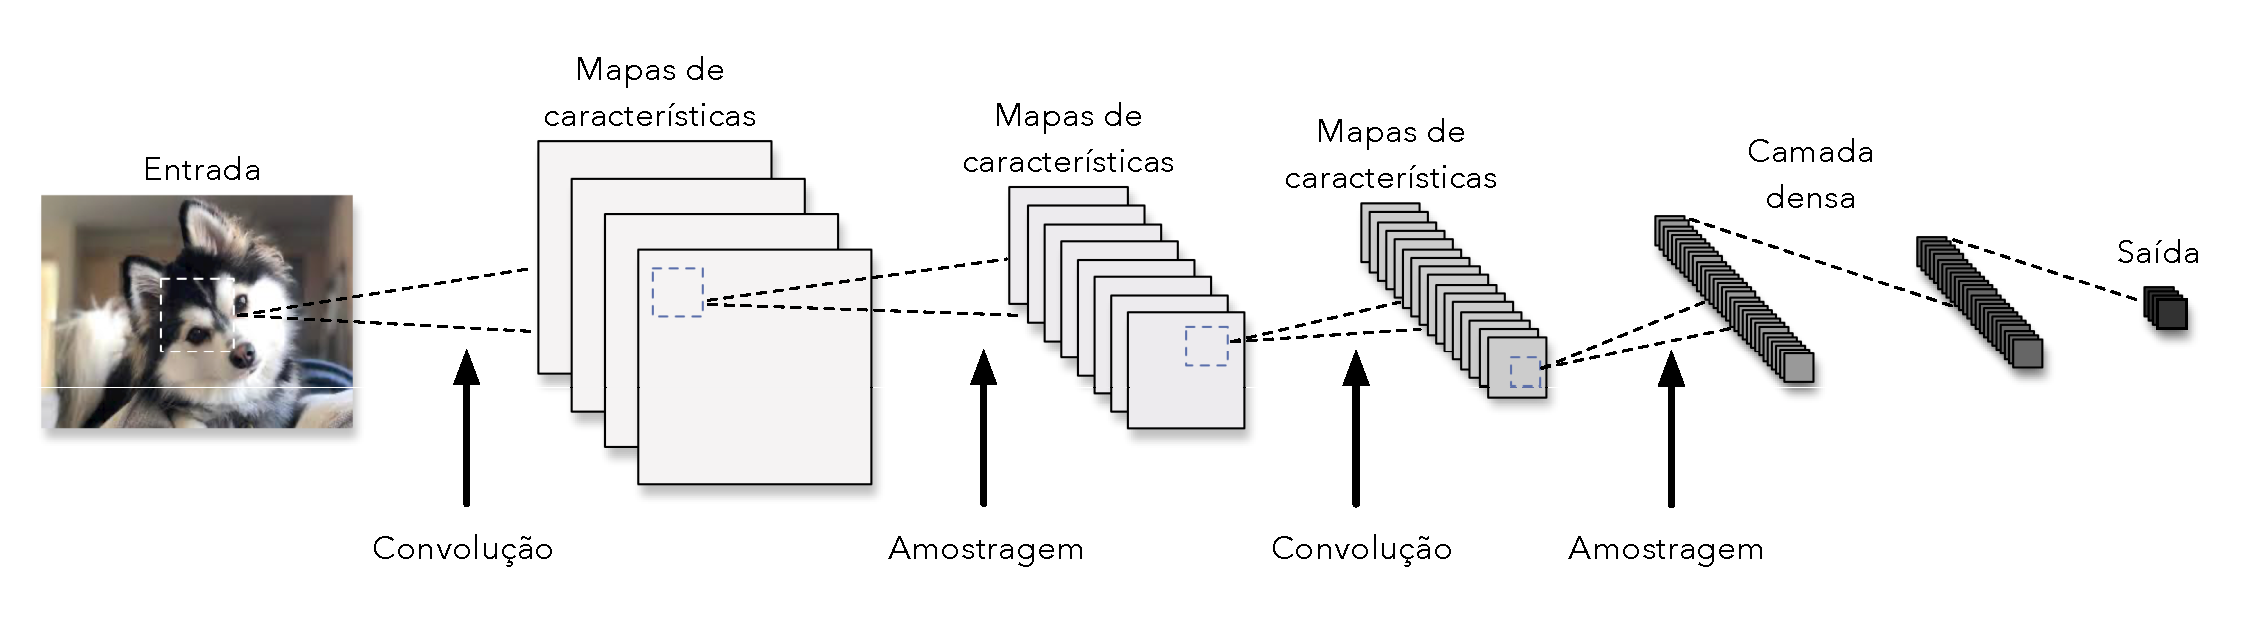
\includegraphics[scale=0.275]{figs/deep_learning.eps}	
		\caption{Exemplo de uma arquitetura multi-camadas de uma Rede Neural Convolucional.}
		\label{f.deep_learning}
	\end{figure}
\end{frame}